% chapter2.tex (Chapter 2 of the thesis)

\chapter{Assessment of Harmonic Based Techniques and Repertoire}

% TODO: Talk about Pythagoreas.
Harmonic based techniques invariably make use of the harmonic series in one way or another. The harmonic series is a sequence of tones in which the frequency of each is an integer multiple of the fundamental frequency. The earliest forms of tuning systems were based around these, but modern instruments are tuned around equal temperament.

\subsection{Background}
Provide an overlay of the techniques and explain how they work, the general benefits and such.
\subsection{Research statement/problem}
Techniques are under-developed and/or under-used.

\subsection{Aim and scope of thesis}
Examples of use in current literature will support use-case scenarios, dearths of usage will support the fact that they are underused.

\subsection{Significance of work}
The production of technique and its uses.

\section{Subharmonics}
% TODO: Explain subharmonics
First discovered by Mari Kimura, subharmonics are a type of overpressure which produces a sound lower than the fundamental.\autocite{kimuraHowProduceSubharmonics1999}  When the bow is drawn across the string, the drag of the bow twists the string, creating torsional oscillation. Under the right conditions, these can interact with the string to produce an identifiable pitch lower than the fundamental.\autocite{Subharmonics2006} \lipsum[3]
\begin{figure}
    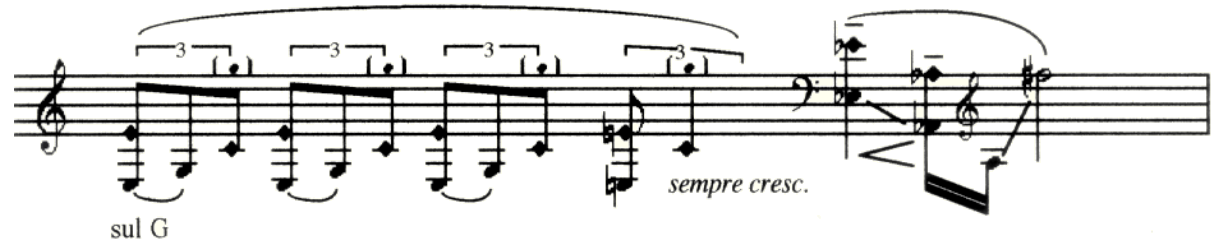
\includegraphics[width=\linewidth]{./resources/kimura_gemini.png}
    \caption{Excerpt from Kimura's Gemini.}
    \label{fig:Excerpt from Kimura's Gemini}
  \end{figure}

\subsection{Works featuring subharmonics}
% TODO: Find pieces using subharmonics
Mari Kimura's `Placeholder' is an example of idiomatic usage of subharmonics on the violin. \lipsum[3]

\section{Multiphonics}
% TODO: Explain multiphonics
Multiphonics on stringed instruments are difficult, but with appropriate preparation and notation, are quite feasible. Production of multiphonics, as with wind instruments, is not guaranteed, and can be dependant on a variety of external factors, including the humidity, make of the instrument, bow used, and other variables that are outside of the control of a composer.

% TODO: Expand Fallowfield discussion.
Fallowfield explores multiphonic production on the cello in her thesis CelloMap.\autocite{fallowfieldCelloMapHandbook2009} \lipsum[2]

\subsection{Works featuring multiphonics}
% TODO: Find multiphonic works
\lipsum[4]

\section{Electronically-Assisted Harmonics}
% TODO: Expand electronic assisted harmonics.
The use of electronics to augment acoustic instruments is hardly a new technique, although their use in a live context is still relatively inaccessible. For my composition `The Veldt', I will be making use of Max MSP, a patch-based audiovisual processing application. 

\subsection{Works featuring electronically assisted harmonics}
% TODO: Find works featuring electronically assisted harmonics
\lipsum[4]
